\section{Einleitung} % (fold)
\label{sec:einleitung}

Bei der Erw"armung einer Metalloberfl"ache ist eine Elektronenemission m"oglich.
Dabei ist besonders die Austrittsarbeit von Bedeutung.
Dabei wird der Versuch im Hochvakuum durchgef"uhrt, damit keine Wechselwirkungen mit den Luftmolek"ulen stattfindet.

\section{Theorie} % (fold)
\label{sec:theorie}

\subsection{Austrittsarbeit und die Energieverteilung} % (fold)
\label{sub:austrittsarbeit_und_die_energieverteilung}

Metalle sind h"aufig kristalline Festk"orper.
Die Atome sind darin ionisiert und die Elektronen geh"oren nicht mehr zu einem bestimmten Atom sondern befinden sich im Kraftfeld s"amtlicher Ionen.
Darin k"onnen sich die Elektronen frei bewegen, wodurch eine hohe elektrische Leitf"ahigkeit erzeugt wird.
Um den Metallverband verlassen zu k"onnen, muss das Elektron gegen das Potential $\psi$ anlaufen k"onnen.
D"af"ur muss die Austrittsarbeit $e_\Mahrm{0}\psi$ geleistet werden.
Das Potential des Gitters kann in grober N"aherung als konstant betrachtet werden.
Abb. \ref{potential_topf} stellt das sogenannte Potentialtopfmodell dar.

\begin{figure}[!h]
	\centering
	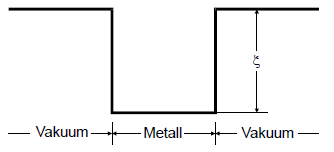
\includegraphics[width = 5cm]{img/Potentialtopf.PNG}
	\caption{Potentialtopfmodell}
	\label{potential_topf}
\end{figure}

Die Elektronen des Kristallgitters unterliegen dem Pauli-Verbot, nach dem nur zwei Elektronen mit entgegengesetztem Spin denselben Zustand mit der Energie $E$ haben k"onnen.
Die Maximalenergie der Elektronen bei T = 0 wird als Grenzenergie $\psi$ bezeichnet.
Die Wahrscheinlichkeit daf"ur, ob ein Zustand mit der Energie $E$ besetzt wird, wird durch die Fermi-Dirac'sche Verteilungsfunktion angegeben:

\begin{equation}
	f(E) = \frac{1}{exp( \frac{E - \psi}{kT} ) + 1} \, .
\end{equation}

Der Verlauf ist in Abb. \ref{fermi} dargestellt.
Die Exponentialfunktion im Nenner "ubertrifft die Zahl 1 bei weitem, wodurch n"aherungsweise gilt:

\begin{equation}
	f(E) \propto exp ( \frac{\psi - E}{kT}) \, .
\end{equation}

\begin{figure}[!h]
	\centering
	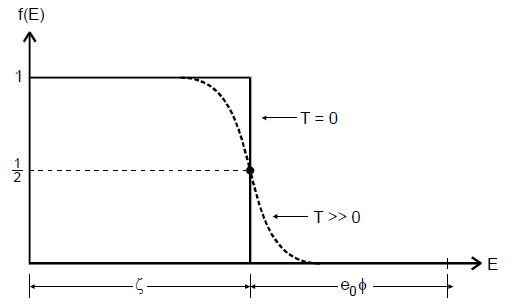
\includegraphics[width = 5cm]{img/Fermi.PNG}
	\caption{Fermi-Dirac'sche Verteilungsfunktion}
	\label{fermi}
\end{figure}

\subsection{Berechnung der S"attigungsstromdichte bei der thermischen Elektronenemission} % (fold)
\label{sub:berechnung_der_s_attigungsstromdichte_bei_der_thermischen_elektronenemission}

F"ur die S"attigungsstromdichte $j_\mathrm{s}(T)$ erh"alt man nach Einf"uhrung eines kartesischen Koordinatensystems:

\begin{equation}
	j_\mathrm{s}(T) = 4\pi \frac{e_\mathrm{0} m_\mathrm{0} k^2}{h^3} T^2 exp( \frac{-e_\mathrm{0} \Phi}{kT}) \, .
\end{equation}

\subsection{Die Hochvakuum-Diode} % (fold)
\label{sub:die_hochvakuum_diode}

Um Wechselwirkungen mit den Gasmolek"ulen der Luft zu vermeiden, muss die Messung des S"attigungsstroms $j_\mathrm{s}$ im Hochvakuum duchgef"uhrt werden.
Diese ist nach Abb. \ref{diode} aufgebaut.
Durch eine angelegte Heizspannung kann die Gl"uhkathode auf 1000 bis 3000\,K erhitzt werden.

\begin{figure}[!h]
	\centering
	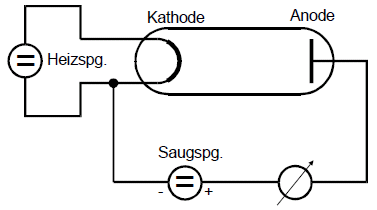
\includegraphics[width = 5cm]{img/Diode.PNG}
	\caption{Beschaltung einer Hochvakuum-Diode}
	\label{diode}
\end{figure}